\documentclass[12pt]{article}

\usepackage[utf8]{inputenc}
\usepackage[margin=1in]{geometry}
\renewcommand{\baselinestretch}{1}
\usepackage{indentfirst}

\usepackage{amsmath, amssymb}

\usepackage{hyperref}
\usepackage{cleveref}
\usepackage{graphicx}
\usepackage{float}
\graphicspath{{./figs/}}

\begin{document}

\begin{center}\begin{LARGE}
\textbf{Assignment 6: Results/Description}
\end{LARGE}\end{center}

\section*{Problem 1}

In this assignment I will be discussing the \texttt{vtop1.f} code. This may be
compiled using \texttt{make vtop1}, shown below:
\begin{figure}[H]
    \centering
    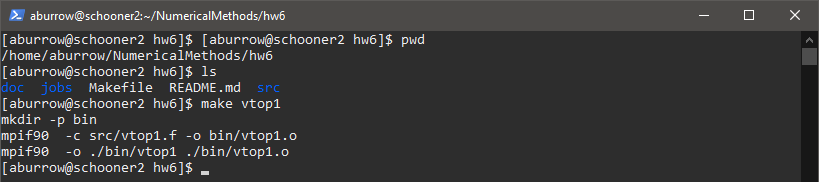
\includegraphics[width=1\textwidth]{compile}
    \label{fig:compile}
\end{figure}
After compiling, this code may be scheduled using \texttt{cd jobs \&\& sbatch
run\_vtop1.slurm} from the root directory. One the job is complete the
resulting output is something like below:
\begin{verbatim}
Calc begins at:  Mon Apr 12 10:13:49 CDT 2021
export LSCRATCH=/lscratch/40757495
 Number of dimensions =            1
 Number of nodes in this dimension =           4
 Periodic F
 My coordinates =           0
 My rank in this communicator =            0
 My coordinates in this linear array           0
 right neighbor           1
 left neighbor          -1
 after exchange (lplace,rplace)           0           1
 Number of dimensions =            1
 Number of nodes in this dimension =           4
 Periodic F
 My coordinates =           1
 My rank in this communicator =            1
 My coordinates in this linear array           1
 right neighbor           2
 left neighbor           0
 Myrank            1 place3
 Number of dimensions =            1
 Number of nodes in this dimension =           4
 Periodic F
 My coordinates =           2
 My rank in this communicator =            2
 My coordinates in this linear array           2
 right neighbor           3
 left neighbor           1
 Myrank            2 place1
 Number of dimensions =            1
 Number of nodes in this dimension =           4
 Periodic F
 My coordinates =           3
 My rank in this communicator =            3
 My coordinates in this linear array           3
 right neighbor          -1
 left neighbor           2
 after exchange (lplace,rplace)           2           0
 after exchange (lplace,rplace)           0           2
 after exchange (lplace,rplace)           1           3
Calc ends at:  Mon Apr 12 10:13:50 CDT 2021
\end{verbatim}

This code shows a basic example of creating and using a virtual topological
communicator, specifically in a Cartesian framework. The idea of this topology
is to allow different processors to communicate more easily as if they were in
a grid, whether this is a 1D, 2D or even a higher-dimensional grid. In this
example code, a 1D framework is created, and it is specified to only work with
4 processes. Therefore a "grid" of 4 processes is a created.

I have annotated each MPI function in this code in more detail. But at its
core, this code creates an MPI environment and creates this topology called
\texttt{MESH\_1D}. Using this grid communicator, each process is able to
extract information about the entire framework (e.g. number of dimensions,
total number of nodes, etc.). Each process can also identify the Cartesian
coordinate rank of itself, as opposed to the global rank you would find using
\texttt{MPI\_COMM\_WORLD}.

Again the benefit of this framework is to allow a system of processors that
acts as a grid. Each processor may easily get the rank of its neighbors through
"shifting". Using these ranks, it can then easily send and receive messages
from these neighbors. In this specific code, this is done to exchange the
values of two variables depending on its left and right neighbors. More
specifically, this is done using tags, which signify that the send/receive
operation is only done when they have the same tag. The output of this code is
quite messy, though, since each process outputs its own result rather than
feeding back into a single master processor.

This functionality may be useful, for example, when you are attempting to model
something with $n$ zones, where the values you are modeling for each zone are
dependent upon those of its neighbors (think of a hydrocode). Then,
theoretically you may just set up a system of processors that represent the
system you are modeling as a grid, and have each processor model a single zone
or even a set of neighboring zones. Each processor may then communicate with
its neighbors as necessary in an easier and possibly more efficient way using
this topology.

\end{document}
